%! Unused graphs

%% Figure Timeline Architecture Image
     \begin{figure}[htb]
          \centering
          % trim=left 190 down 250 right 150 top5
          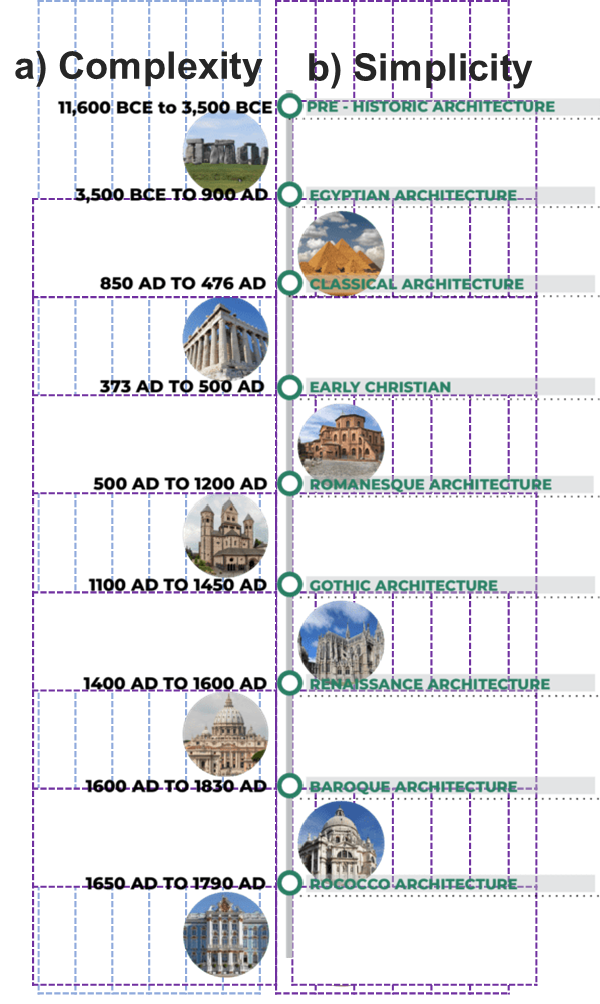
\includegraphics[width= \linewidth]{Images/TimelineArchitecture}
          \caption{Timeline of Architecture and the recurrent pattern of complexity and simplicity}
          \label{fig:TimelineArchitecture}
        \end{figure}

%%Figure Romanesque vs Gothic figure
     \begin{figure}[htb]
          \centering
          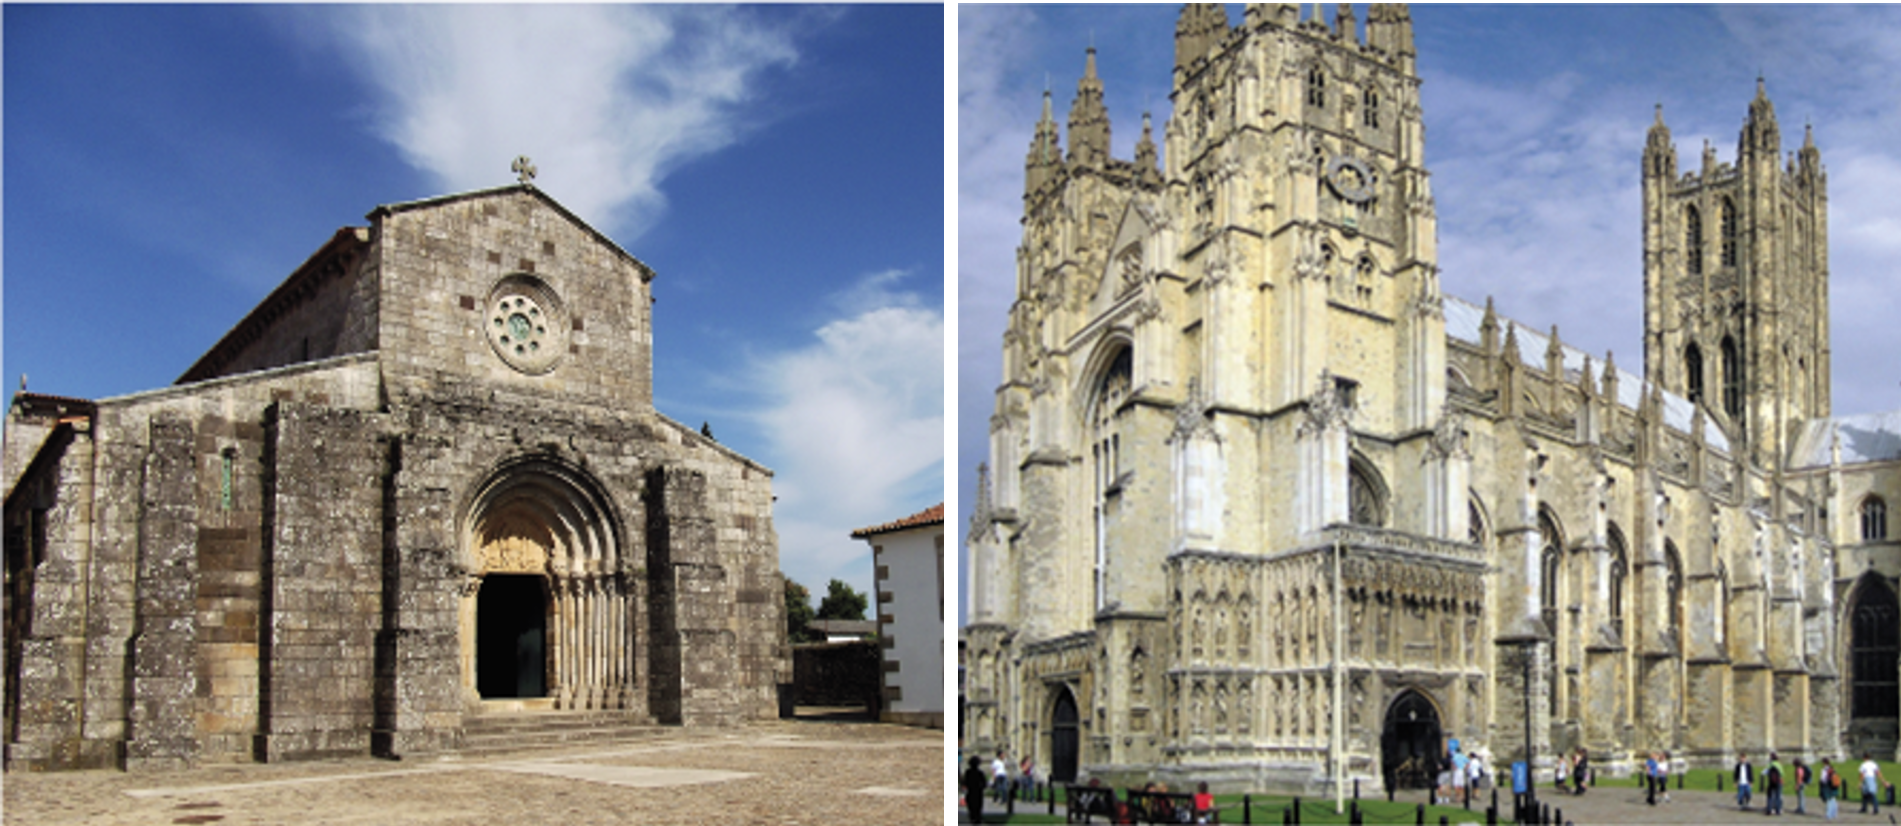
\includegraphics[width= \linewidth]{Images/RomanesqueVsGothic}
          \caption{Romanesque Church 10th AC (left) vs Gothic church 12th AC (right). From simplicity to complexity. (\textit{Images edited from source})}
          \label{fig:RomanesquevsGothic}
        \end{figure}

%%Figure ArtNouvau vs Modernism
     \begin{figure}[htb]
          \centering
          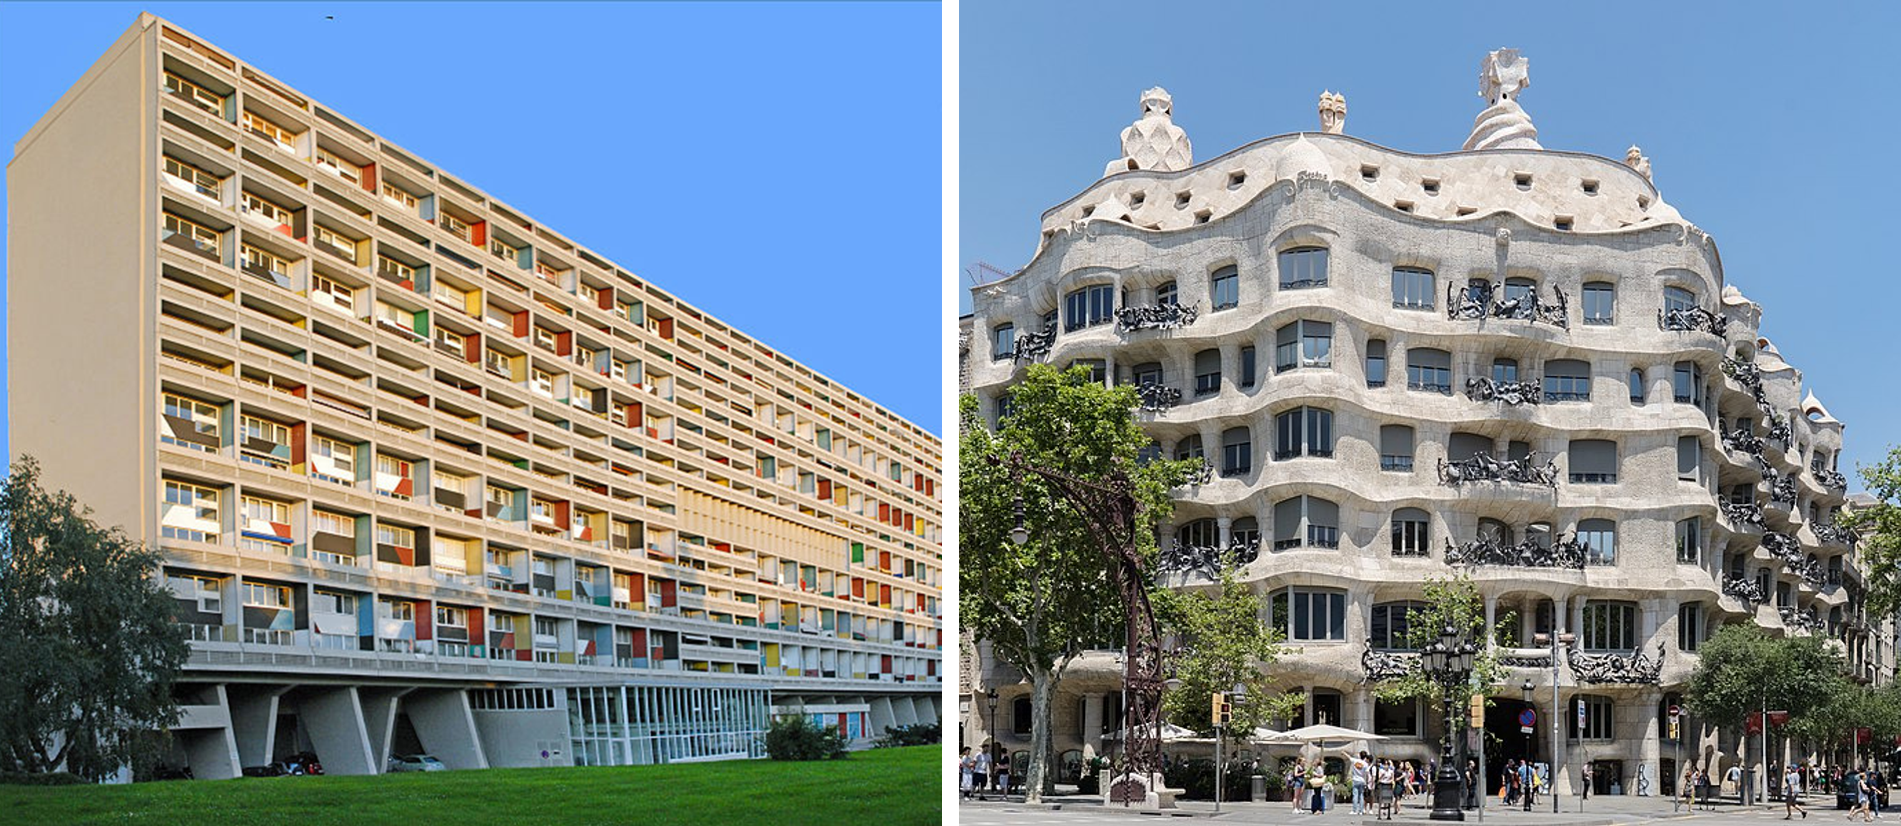
\includegraphics[width= \linewidth]{Images/ArtNouveauVsModernism}
          \caption{Modern Architecture 20th century (Left) vs Art Nouveau building 1920's 30's (Right). To simplicity from complexity. (\textit{Images edited from source})}
          \label{fig:ArtNouveauVsModernism}
        \end{figure}

%%Figure Modernism vs contemporary
     \begin{figure}[htb]
          \centering
          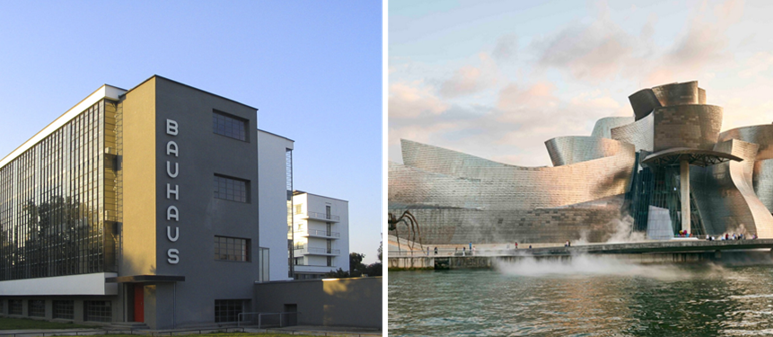
\includegraphics[width= \linewidth]{Images/modernism vs postmodernism}
          \caption{Modernist building "Bauhaus School" 20th AC (left) vs Postmodernist "Guggenheim museum" 1997 (right). From simplicity to Complexity. (\textit{Images edited from source:\cite{Arora2023}})}
          \label{fig:Modernismvscontemporary}
        \end{figure}

%%Figure neoclassicim vs modernism
     \begin{figure}[htb]
          \centering
          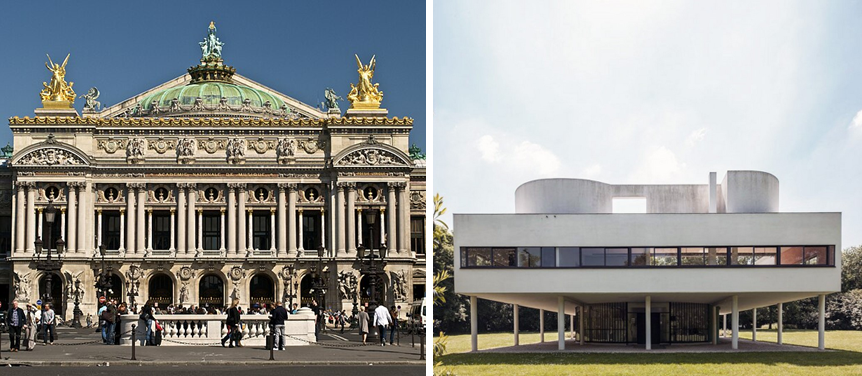
\includegraphics[width= \linewidth]{Images/NeoclassicismVsModernism}
          \caption{Neoclassic building "Paris Opera" 19th AC (left) vs Modernist house "Villa Savoye" 20th AC (right). From Complexity to simplicity. (\textit{Images edited from source:\cite{Stacbond2020}})}
          \label{fig:NeoclassicalvsModernism}
        \end{figure}

    %% Figure of baroque facade vs contemporary facade
    \begin{figure}[htb]
        \centering
        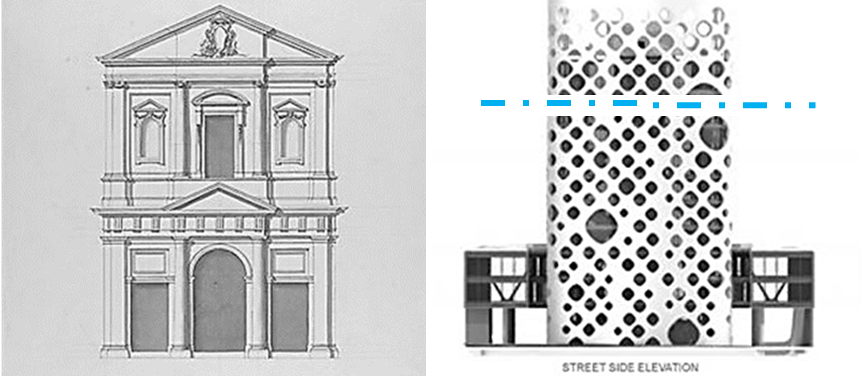
\includegraphics[width= \linewidth]{Images/BaroqueVsContemporaryfacade}
        \caption{Evolution of facade design.
        Baroque Facade 1639 by Bernini (left) vs Contemporary facade, building O-14 by Reiser + Umemoto, 21st Century (right). (\textit{Images edited from source})}
        \label{fig:FacadeBaroqueVsContemporary}
    \end{figure}

    %% Figure of Vitruvian Architecture
    \begin{figure}[htb]
    \centering
    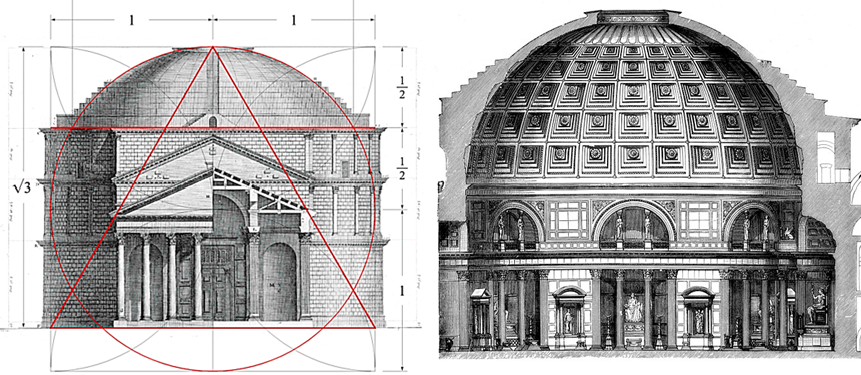
\includegraphics[width= \linewidth]{Images/VitruvianArchitecture}
    \caption{Facade and ornament according to Vitruvius, with emphasis on order, symmetry, and harmony. Pantheon's facade (left) and cross-section (right) symmetry analysis. (\textit{Images edited from source})}
    \label{fig:Vitruvianarchitecture}
    \end{figure}

    %% Figure of Baroque facade Borromini
    \begin{figure}[htb]
    \centering
    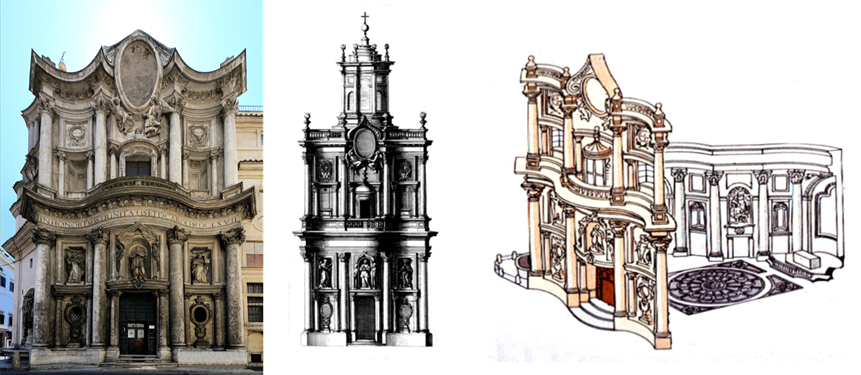
\includegraphics[width= \linewidth]{Images/BaroquefacadeBorromini}
    \caption{Borromini's Interpretation of Facade and Ornament: Elaborate geometric patterns, curved forms, and sculptural elements reflecting internal spatial arrangements. Analysis of San Carlo alle Quattro Fontane Church Facade (left) and Cross Section (right) from its construction in the 1630s, Rome. (\textit{Images edited from source})}
    \label{fig:BorrominiArchitecture}
    \end{figure}

    %% Figure of Classicism and Neo-Classicism facade
    \begin{figure}[htb]
    \centering
    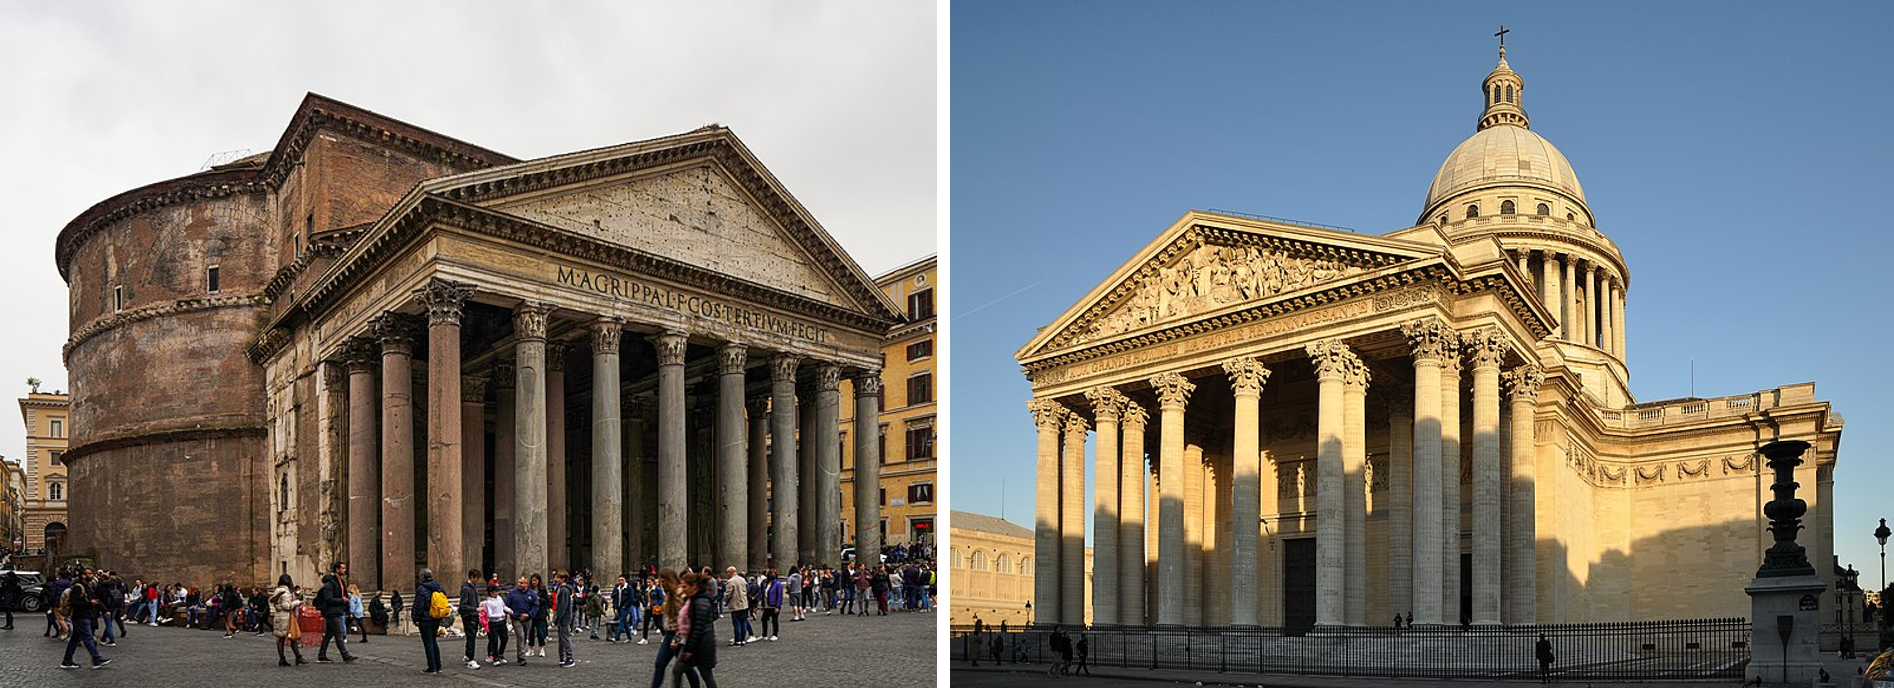
\includegraphics[width= \linewidth]{Images/ClassicismNeoClassicism}
    \caption{Neo-Classical Facades: Emphasis on formal elegance and symmetry. (Left) Pantheon in Rome, 27 BC. (Right) Pantheon in Paris, 1758-1790, Neoclassical style. (\textit{Images edited from source})}
    \label{fig:ClassicismNeoClassicism}
    \end{figure}

    %% Figure of Art Nouveau style facade
    \begin{figure}[htb]
    \centering
    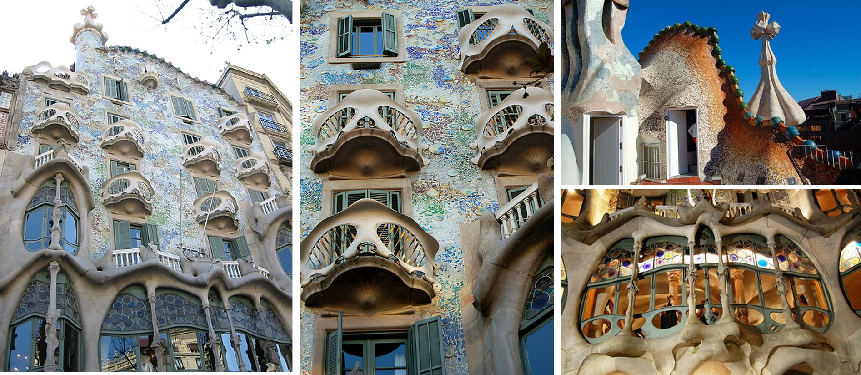
\includegraphics[width= \linewidth]{Images/ArtnouveauGaudi}
    \caption{Art Nouveau Style: Organic forms and nature-inspired motifs. Casa Batlló by Gaudi, 1904. (\textit{Images edited from source})}
    \label{fig:ArtNouveaustyle}
    \end{figure}

    %% Figure of Art Deco style facade
    \begin{figure}[htb]
    \centering
    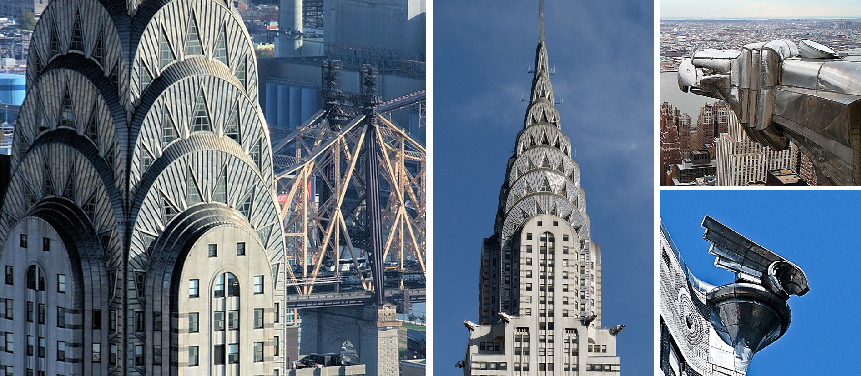
\includegraphics[width= \linewidth]{Images/ArtDecoFacade}
    \caption{Art Deco: Fusion of modernity and historical nostalgia. Chrysler Building, 1930. (\textit{Images edited from source})}
    \label{fig:ArtDeco}
    \end{figure}

    %% Figure of Art Nouveau style facade
    \begin{figure}[hb]
    \centering
    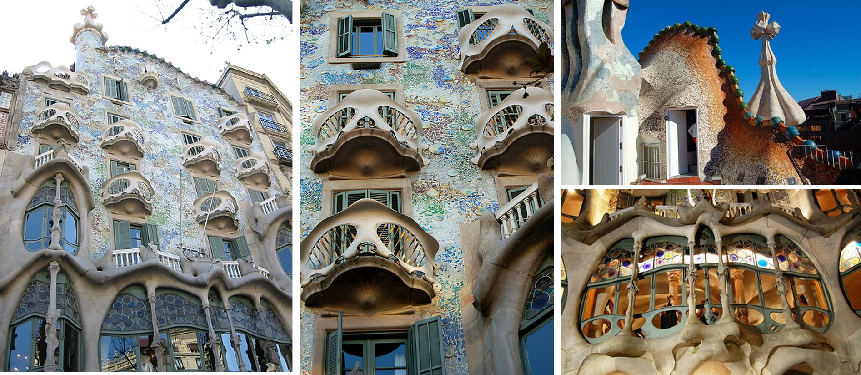
\includegraphics[width= \linewidth]{Images/ArtnouveauGaudi}
    \caption{Art Nouveau Style: Organic forms and nature-inspired motifs. Casa Batlló by Gaudi, 1904. (\textit{Images edited from source})}
    \label{fig:ArtNouveaustyle}
    \end{figure}

    %% Figure of Art Deco style facade
    \begin{figure}[hb]
    \centering
    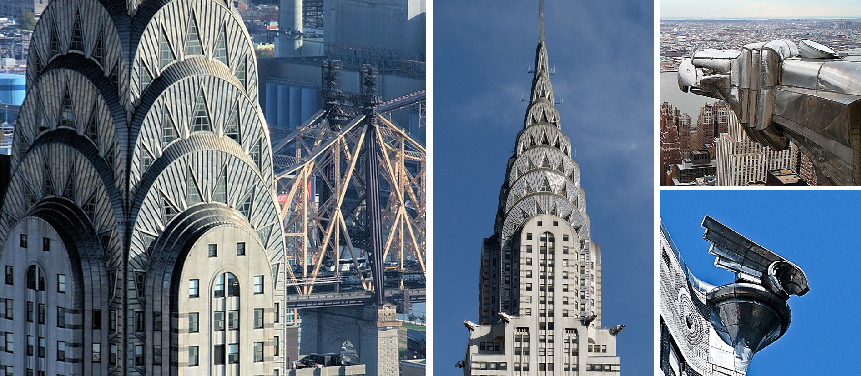
\includegraphics[width= \linewidth]{Images/ArtDecoFacade}
    \caption{Art Deco: Fusion of modernity and historical nostalgia. Chrysler Building, 1930. (\textit{Images edited from source})}
    \label{fig:ArtDeco}
    \end{figure}

    %% Figure of Modernist facade and ornament by Le Corbusier
    \begin{figure}[htb]
        \centering
        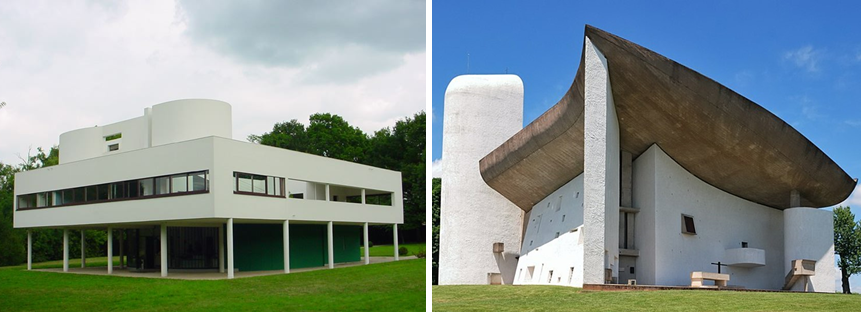
\includegraphics[width= \linewidth]{Images/ModernistFacade}
        \caption{Functionalism in Modernist Facade Design: Le Corbusier's approach. (Left) Villa Savoye, 1928--1931. (Right) Chapelle Notre-Dame-du-Haut de Ronchamp, 1955. (\textit{Images edited from source})}
        \label{fig:Modernistfacade}
    \end{figure}

    %% Figure of Postmodernism ornament
    \begin{figure}[htb]
        \centering
        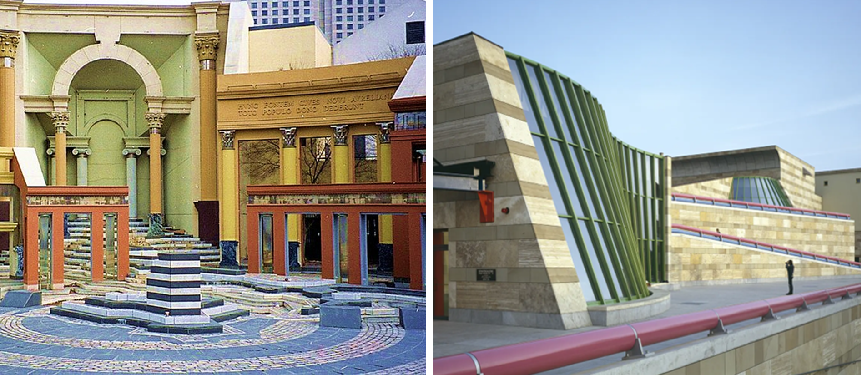
\includegraphics[width= \linewidth]{Images/PostmodernOrnament}
        \caption{Postmodernism's Diverse Ornamentation: (Left) Piazza d’Italia, 1978. (Right) Neue Staatsgalerie, 1984. (\textit{Images edited from source})}
        \label{fig:postmodernOrnamnet}
    \end{figure}

%% Figure of Postmodernism facade and ornament
\begin{figure}[htb]
\centering
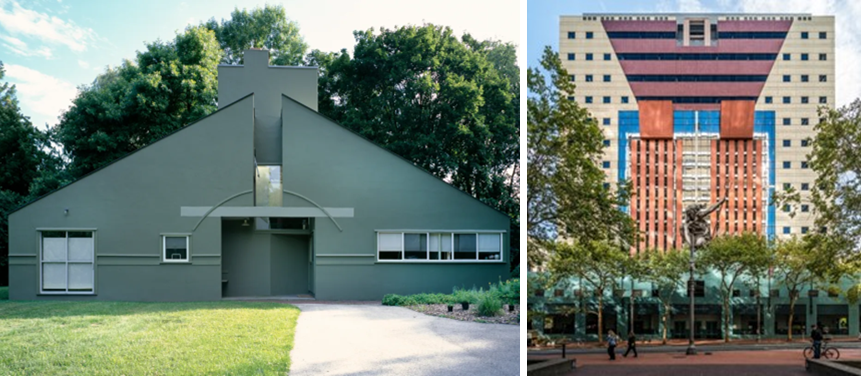
\includegraphics[width= \linewidth]{Images/PostmodernismVenturi}
\caption{Postmodernism's Complexity and Contradiction: (Left) Vanna Venturi House, 1964. (Right) Portland Municipal Services Building, 1982. (\textit{Images edited from source})}
\label{fig:postmodernfacade}
\end{figure}

Similarly, the elaborate Art Deco architecture of the 1920s stands in stark contrast to the subsequent embrace of simplicity of Modern Architecture and rationalism  of the mid-20th century that championed functionalism and minimalist aesthetics, showcasing innovative materials like steel, glass, and concrete\cite{Stacbond2020}(see Figure\ref{fig:ArtNouveauVsModernism}).



%! Original alternative for accuracy graphs alternative


 %% Figure Complexity perception per level with trendlines
    \begin{figure*}[htb]
      \centering
      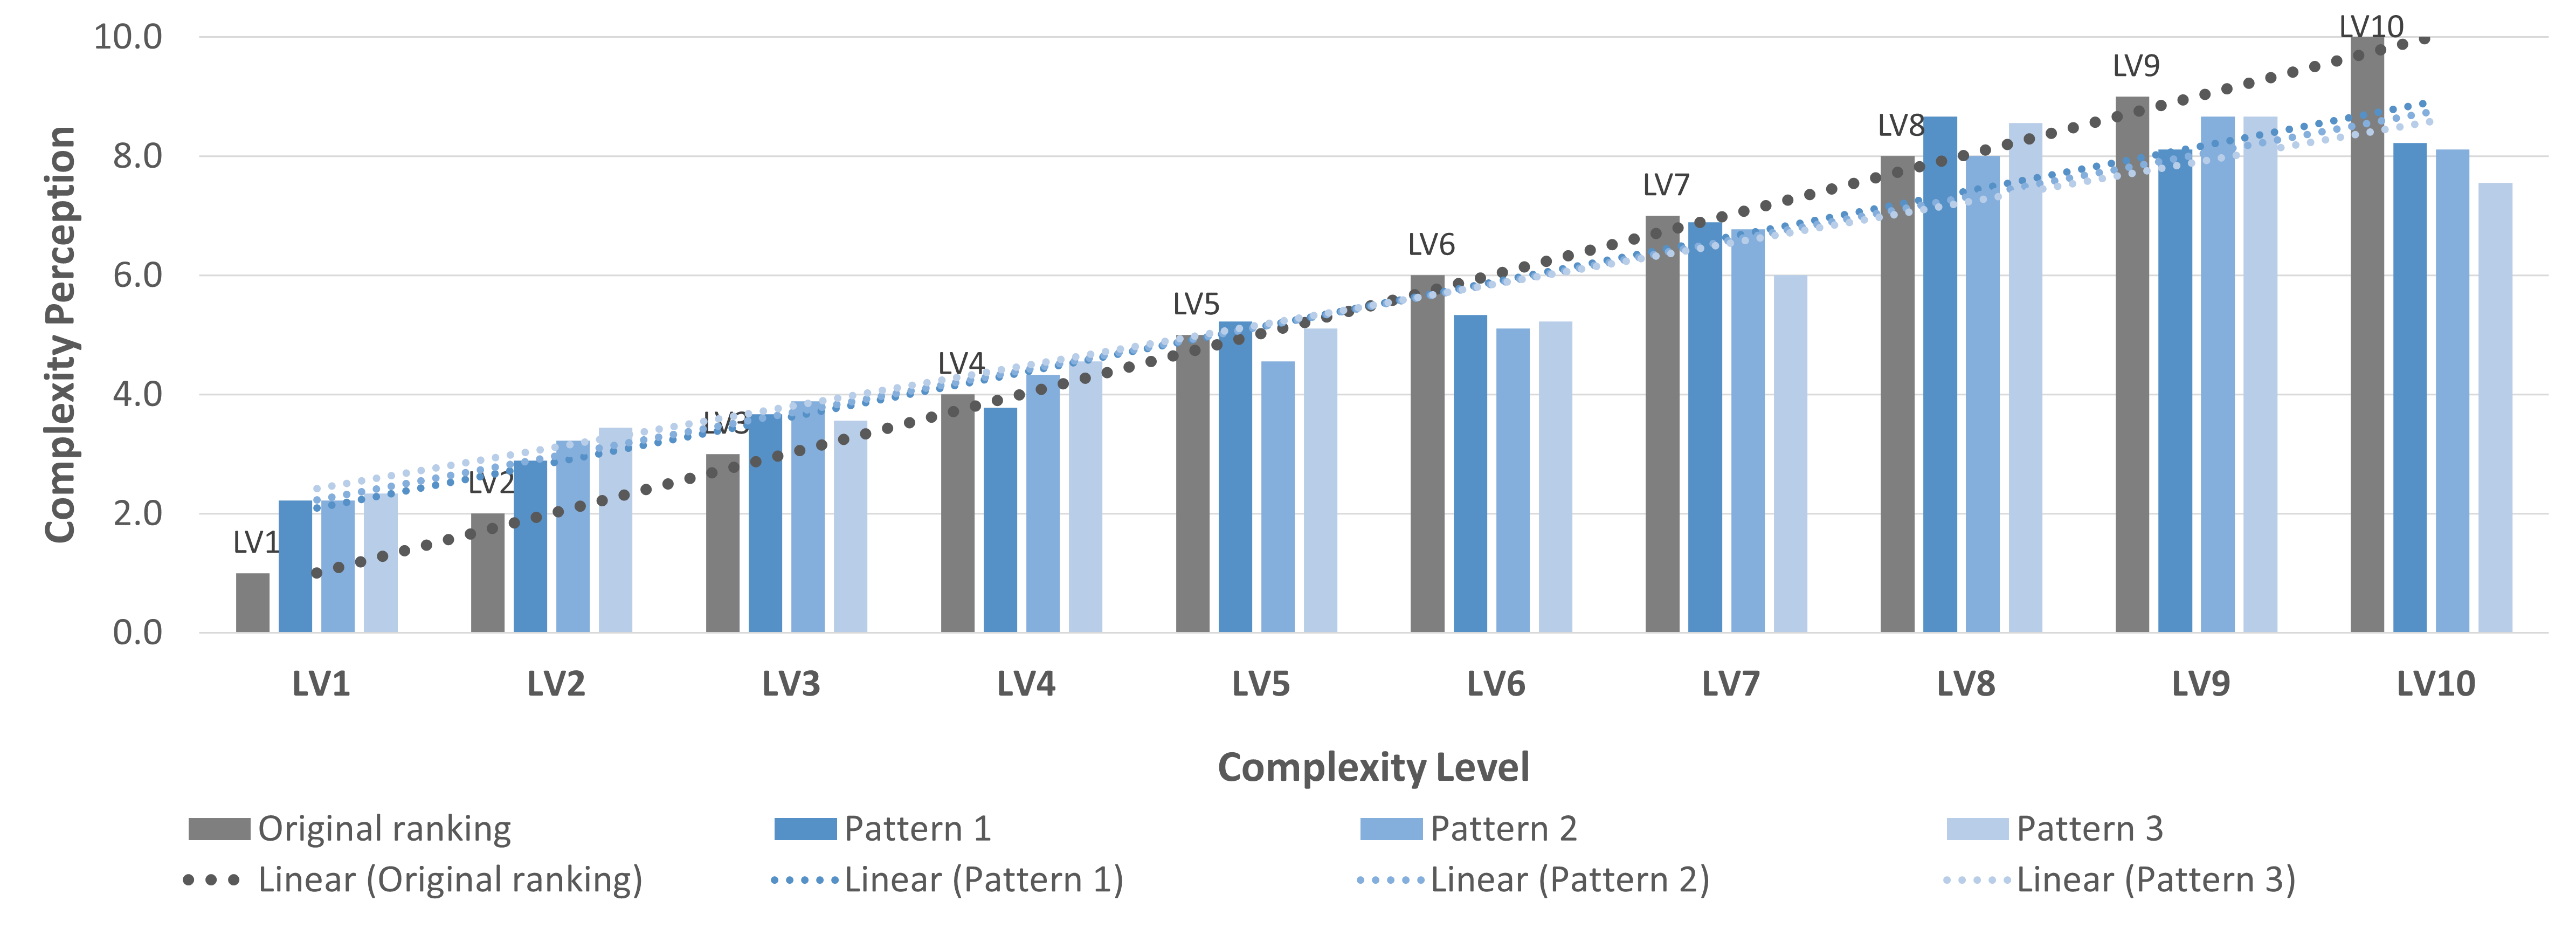
\includegraphics[width= \linewidth, trim=0 0 0 0]{Images/ComplexityPerceptionPerLevel}
      \caption{This graph highlights participants' perception of complexity for the 10 variations within three patterns in contrast to the original ranking. It visually represents the differences between participants' perceived complexity and the initial rankings during the screen-based complexity assessment stage of the experiment.}
      \label{fig:ComplexityPerceptionPerLevel2}
    \end{figure*}

% Old Figure Complexity perception Chart for all patterns
    \begin{figure}[htb]
        \centering
        %trim=100 180 100 120, clip
        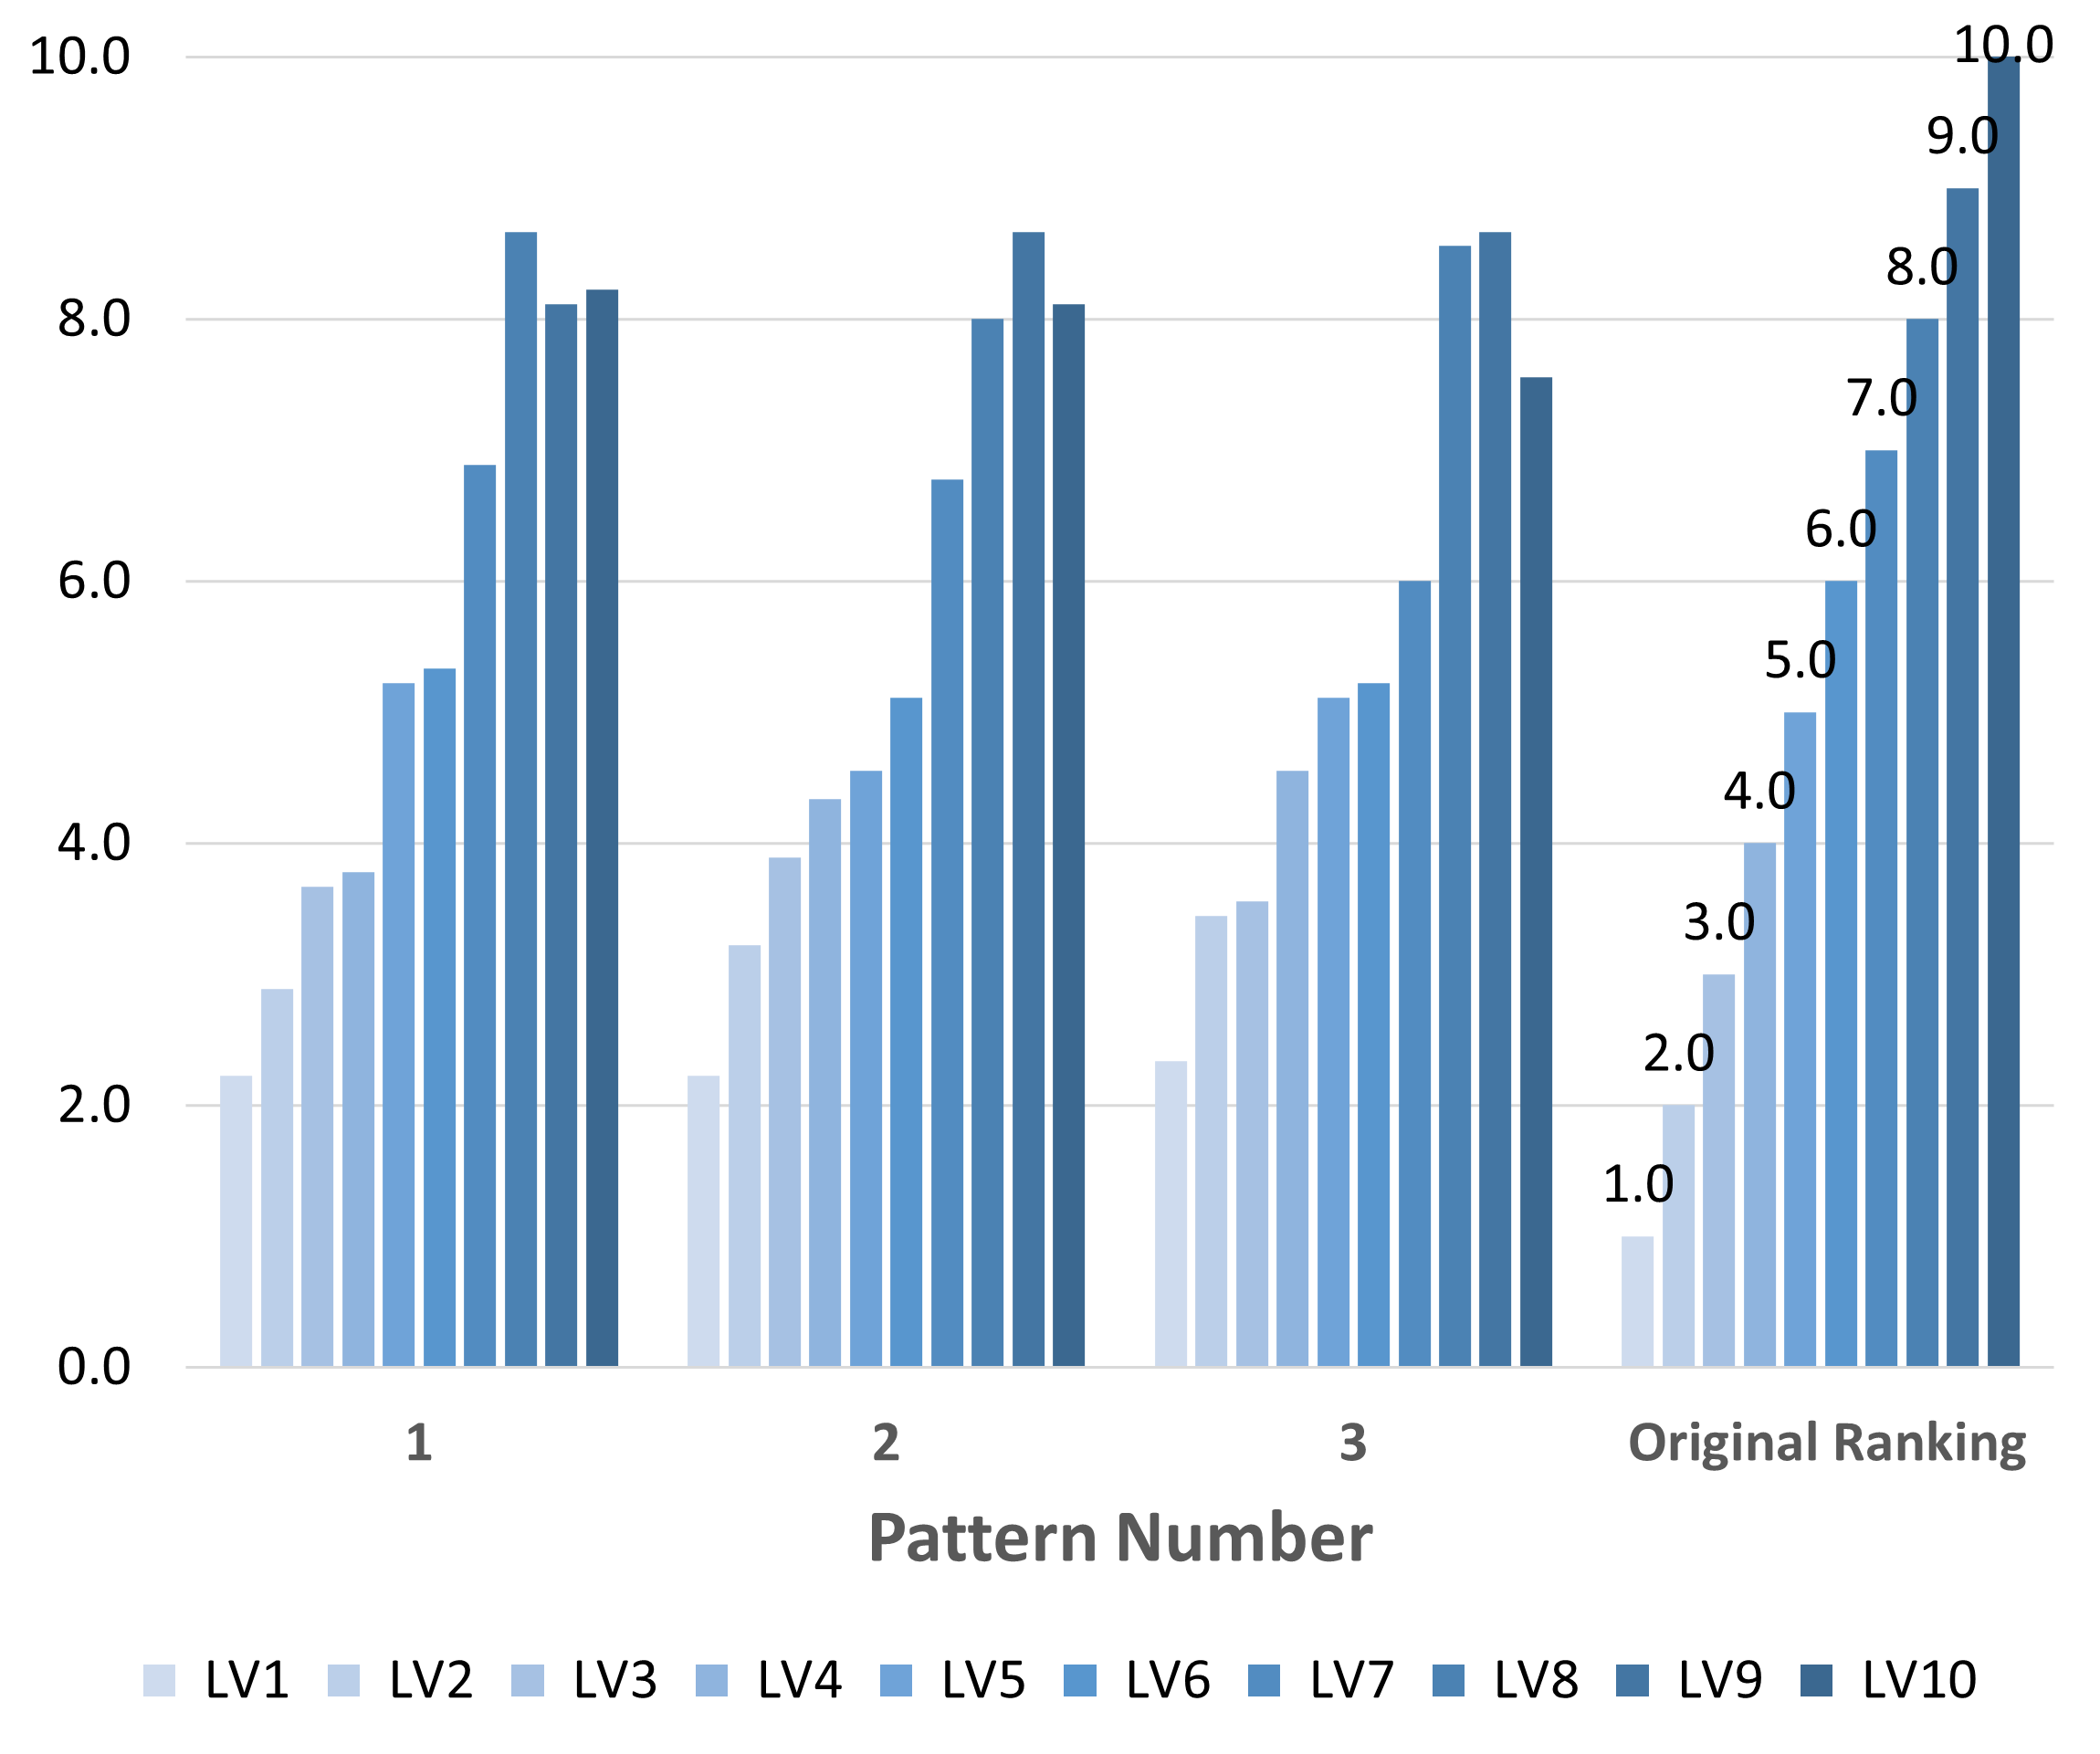
\includegraphics[width=\linewidth]{Images/ComplexityPerceptionChart}
        \caption{Chart depicting participants' complexity perception related to the three patterns. Insights into participants' perception of complexity concerning specific patterns during the screen-based complexity assessment phase of the experiment.}
        \label{fig:ComplexityPerceptionChart}
    \end{figure}


%! Future ornament graph

(Figure \ref{fig:complexornament})

%% Figure of Contemporary timeline
     \begin{figure*}[htb]
          \centering
          \includegraphics[width= \linewidth]{Images/complexornament}
          \caption{Complex ornament reference  (\textit{Images edited from source)}}
          \label{fig:complexornament}
        \end{figure*}


%! Texts

    %In Complexity and Contradiction in Architecture, Robert Venturi tries to give counter-arguments to the modernist approach. He advocates embracing ‘contradiction and Images’ to create valid, vital works.\cite{Lutolli2020}


    %It is noteworthy that he doesn’t oppose aesthetic simplicity. What he rejects is the ‘oversimplification’ of architecture, indicated when he inverted the famous Mies van der Rohe statement ‘Less is more’ into ‘Less is a bore’.\cite{Lutolli2020}

    %Modern architects, who shunned symbolism of form  as  an expression or reinforcement of content: meaning was  to  be  communicated,  not  through  allusion  to  previously  known forms, but through the inherent, physiognomic characteristics of form.
    %The creation of architectural form was to be a logical process, free  from images  of past experiences, determined solely by program and structure, with an  occasional  assist,  as  Alan Colquhoun has  suggested, from  intuition.
    But some recent critics  have  questioned  the possible level of content to  be derived  from  abstract forms.
    Others have  demonstrated that the functionalists,  despite  their protestations, derived  a  formal vocabulary of their own, mainly from current art movements and the industrial vernacular;
    and  latter-day  followers  such  as  the  Archigram  group  have turned,  while  similarly  protesting,  to Pop  Art and  the space  industry.\cite{Venturi1972}

   % Because the spatial relationships are made by symbols more than by forms, architecture in this landscape becomes symbol in space rather than form in space.
    Architecture defines very little: The big sign and the little building is the rule of Route 66.
    %The sign is more important than the architecture.
    %This is reflected in the proprietor's budget the sign at the front is a vulgar extravaganza, the building at the back, a modest necessity.
    The architecture is what is cheap.\cite{Venturi1972}

    %The commercial persuasion of road­side eclecticism provokes bold impact in the vast and complex setting of a  new landscape of big spaces, high speeds, and complex programs.\cite{Venturi1972}

    %parking lot is a current phase in the evolution of vast space since Versailles (Fig. 12). The space that divides high-speed highway and low, sparse buildings produces no enclosure and Iittle direction. \cite{Venturi1972}

    The little low buildings, gray-brown like the desert, separate and recede from the street that is now the highway, their false fronts disengaged and turned perpendicular to the highway as big, high signs.
    If you take the signs away, there is no place.
    The desert town is intensified communication along the highway.\cite{Venturi1972}

    Ugly and ordinary as symbol and style
    Heroic and Original, or ugly and ordinary

    %Robert Venturi, an iconoclastic architect often considered the father of postmodernism who rejected sterile, glass-cube structures in favor of an inclusive, eclectic style that embraced community values and a touch of vulgarity\cite{Schudel2018}

    He turned Mies van der Rohe’s famous dictum about simplicity in design — “Less is more” — upside down, cheekily declaring, “Less is a bore.”\cite{Schudel2018}

    Mr. Venturi’s declaration of architectural values, “Complexity and Contradiction,” was a manifesto that took aim at the prevailing modernist notion that architecture should aspire to a cold, glassy perfection with cold, glassy buildings.
    He argued instead that architecture should reflect changing times and social needs.
    The world of design, he said, had too long been in the grip of the dogma that architects were godlike creators who could impose their vision on the landscape.\cite{Schudel2018}

     Las Vegas wasn’t just a neon-lit den of vulgarity, they concluded.
     It was a prime example of a city built to accommodate the automobile.
     As a result, signs were often more important than the buildings they loomed over.\cite{Schudel2018}

    “In the landscape of the automobile, the architecture becomes insignificant, a pimple on the landscape of parking lots,” Mr. Venturi told the Times in 1971.\cite{Schudel2018}

    He never lost his disdain for what he considered the soulless architecture of his modernist predecessors, who often designed glass-box buildings with walls of windows, “but you would never have a wall with a window in it.”\cite{Schudel2018}

    Instead, Mr. Venturi wrote in “Complexity and Contradiction in Architecture,” he drew inspiration from the “everyday landscape, vulgar and disdained,” which was “valid and vital for our architecture as a whole.”\cite{Schudel2018}

    some architects wanted to move away from minimalist glass and steel and return to the ornamentation of the past. Postmodernists such as Michael Graves, James Stirling, Robert Venturi, and Denise Scott Brown responded to the work of their predecessors with bold buildings that showcased color and references to classical design. [...] Discover five of the most influential buildings of the postmodern movement and see how their eclectic and innovative designs pushed the boundaries of architecture in the 20th century\cite{Stamp2016}.

    Venturi wants modern architects to realize only one thing— perfection in the architectural world can and should include imperfection, in all its forms\cite{Lutolli2020}.

    %Modern architecture submerged symbolism. Instead it promoted expressionism, concentrating on the expression of architectural elements themselves: on the expression of structure and function\cite{Venturi1971}

    %Modern architecture's expression has become a dry expressionism, empty and boring. And in the end, irresponsible: i ron i c a I I y the Modern architecture of Crawford Manor, while rejecting explicit symbolism and frivolous applique ornament, has distorted the whole building into one big ornament\cite{Venturi1971}.

     Modern architects, who shunned symbolism of form  as  an expression or reinforcement of content: meaning was  to  be  communicated,  not  through  allusion  to  previously  known forms, but through the inherent, physiognomic characteristics of form.
    The creation of architectural form was to be a logical process, free  from images  of past experiences, determined solely by program and structure, with an  occasional  assist,  as  Alan Colquhoun has  suggested, from  intuition.
    But some recent critics  have  questioned  the possible level of content to  be derived  from  abstract forms.
    Others have  demonstrated that the functionalists,  despite  their protestations, derived  a  formal vocabulary of their own, mainly from current art movements and the industrial vernacular;
    and  latter-day  followers  such  as  the  Archigram  group  have turned,  while  similarly  protesting,  to Pop  Art and  the space  industry.\cite{Venturi1972}

    %
    According to Krier the mature city achieves balance with nature and with the people that it serves in its scale, size and integration of residential, commercial and civic functions.
    Krier argues that the reconstruction of a city is a moral imperative, a global project that it is at once cultural social economic and ecological. Time of video 1:06:29\cite{Economakis2023}